\documentclass[%
reprint,
%superscriptaddress,
%groupedaddress,
%unsortedaddress,
%runinaddress,
%frontmatterverbose, 
%preprint,
%preprintnumbers,
nofootinbib,
%nobibnotes,
%bibnotes,
 amsmath,amssymb,
aps,
%pra,
%prb,
%rmp,
%prstab,
%prstper,
%floatfix,
superscriptaddress,
showkeys,
%endfloats,
%onecolumn,
longbibliography
]{revtex4-1}

%TESTE
\usepackage{enumitem}

\usepackage{xr}
\usepackage{tabularx}
\usepackage{booktabs}
\usepackage{graphicx}% Include figure files
\usepackage{dcolumn}% Align table columns on decimal point
\usepackage{bm}% bold math
\usepackage{microtype}
\usepackage{gensymb}
\usepackage{url}
\usepackage[breaklinks, hidelinks, colorlinks=true,linkcolor=blue,citecolor=black]{hyperref}% add hypertext capabilities
\usepackage{color, colortbl}
\usepackage[table,xcdraw]{xcolor}
%\usepackage[mathlines]{lineno}% Enable numbering of text and display math
%\linenumbers\relax % Commence numbering lines

%\usepackage[showframe,%Uncomment any one of the following lines to test 
%%scale=0.7, marginratio={1:1, 2:3}, ignoreall,% default settings
%%text={7in,10in},centering,
%%margin=1.5in,
%%total={6.5in,8.75in}, top=1.2in, left=0.9in, includefoot,
%%height=10in,a5paper,hmargin={3cm,0.8in},
%]{geometry}

%VER
\usepackage[table]{xcolor}

\makeatletter
\renewcommand\frontmatter@abstractwidth{\dimexpr0.9\textwidth\relax}
\makeatother


% \bibliographystyle{apsrev4-1}
\usepackage{algorithm}
\usepackage{algpseudocode}

\makeatletter
\newcommand*{\addFileDependency}[1]{% argument=file name and extension
  \typeout{(#1)}
  \@addtofilelist{#1}
  \IfFileExists{#1}{}{\typeout{No file #1.}}
}
\makeatother

\newcommand*{\myexternaldocument}[1]{%
    \externaldocument{#1}%
    \addFileDependency{#1.tex}%
    \addFileDependency{#1.aux}%
}

\newcommand{\sm}{\scalebox{0.5}[1.0]{\( - \)}}


%VER
\makeatletter
\renewcommand\subparagraph{\@startsection{subparagraph}{5}{\parindent}%
    {3.25ex \@plus1ex \@minus .2ex}%
    {-1em}%
    {\normalfont\normalsize\bfseries}}
\makeatother

\begin{document}

\preprint{1}



\title{VessShape: Few-shot blood vessel segmentation by leveraging shape priors from synthetic images}
%VessShape: Few-shot blood vessel segmentation using shape priors from synthetic data
%VessShape: Adding shape priors to neural networks for few-shot blood vessel segmentation

\author{Wesley Nogueira Galvão}
\affiliation{Department of Computer Science, Federal University of S\~ao Carlos, S\~ao Carlos, SP, Brazil}


\author{Cesar H. Comin}
\email[Corresponding author: ]{comin@ufscar.br}
\affiliation{Department of Computer Science, Federal University of S\~ao Carlos, S\~ao Carlos, SP, Brazil}

\date{\today}% It is always \today, today,
             %  but any date may be explicitly specified

\begin{abstract}

??

\end{abstract}

\keywords{Blood vessel segmentation, Connectivity, post-processing}

\maketitle
\thispagestyle{plain}
%\ohead*{\pagemark}

\section{Introduction}
\label{sec:introduction}



\section{Related Works}
\label{sec:related}

- Pre-training with synthetic data

- Synthetic data in medical images

- Shape priors for medical images segmentation using neural networks

- Shape priors for vessel segmentation (classic methods)

- Shape priors for vessel segmentation (neural networks)

\section{Methodology}
\label{s:methodology}

\subsection{VessShape}

VessShape is a synthetic image dataset that combines tubular, vessel-like shapes with diverse foreground and background textures. The central idea is to provide a robust set that can be used to train blood vessel segmentation models while keeping geometric priors fixed and drastically changing texture, encouraging models to learn shape cues (connectivity, tapering, bifurcations) rather than overfitting to texture.

The geometry of this dataset is based on Bézier curves, which allow a flexible and controlled representation of tubular shapes. Each vascular branch $C_k$ is described by an $n$-th order Bézier curve with control points $\{\mathbf{P}_{k,i}\}_{i=0}^n$, sampled to produce connected branches and plausible bifurcation angles. Tortuosity is adjusted by small perturbations to the control points, ensuring that vessel geometry is realistic and diverse.

\begin{equation}
\mathbf{c}_k(t) \,=\, \sum_{i=0}^{n} \binom{n}{i} (1-t)^{n-i} t^{i} \, \mathbf{P}_{k,i}, \qquad t \in [0,1].
\label{eq:bezier}
\end{equation}

\begin{table*}[t]
\caption{VessShape generation parameters, sampling ranges, and description.}
\label{tab:vessshape_params}
\centering
\begin{tabularx}{\textwidth}{l c X}
\hline
    \textbf{Parameter} & \textbf{Range} & \textbf{Description} \\
\hline
Number of curves $K$ & $[1,20]$ & Number of branches/vessels generated per sample. \\
Control points $n{+}1$ & $[2,20]$ & Bézier curve complexity (order $n$). \\
Displacement scale $\delta$ (px) & $[50.0,150.0]$ & Controls curvature/tortuosity via the typical amplitude of control-point displacement. \\
Initial radius $r_{0,k}$ (px) & $[1,5]$ & Basal vessel thickness; a smooth taper is applied along the branch. \\
Matting blur $\sigma$ & $[1,2]$ & Standard deviation of the Gaussian used for $A = G_{\sigma} * M$. \\

\hline
\end{tabularx}
\end{table*}

\begin{equation}
I(x) \,=\, A(x)\,F(x) + (1-A(x))\,B(x), \qquad x \in \Omega.
\label{eq:compose}
\end{equation}

\subsection{Training details}

\subsection{Fine-tuning}

- Datasets (VessMAP e DRIVE)

- Procedure

\section{Results}
\label{s:results}

\begin{figure*}[tbp]
    \centering
    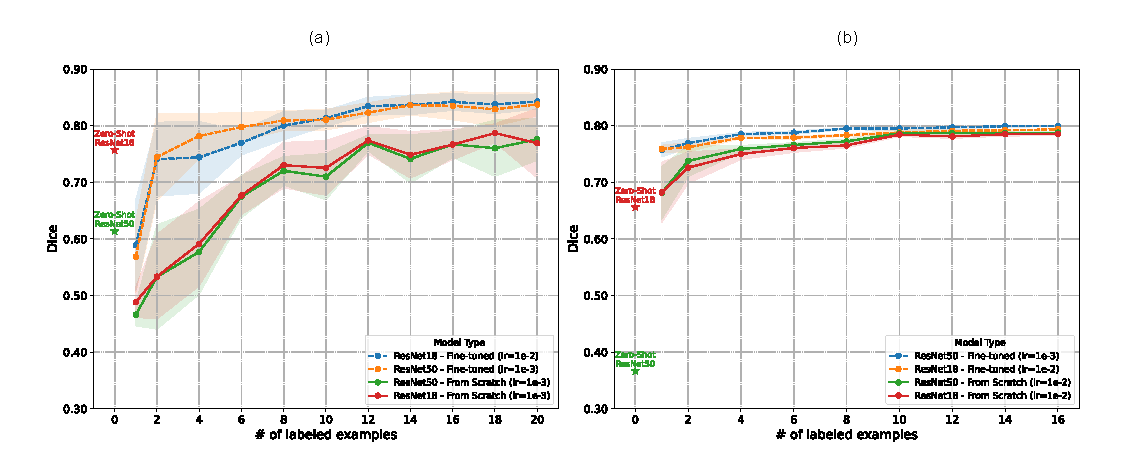
\includegraphics[width=\textwidth]{figures/results/results_charts_normalized.pdf}
    \caption{??.}
    \label{f:results_charts_normalized}
\end{figure*}


\begin{table*}[t]
\caption{Zero-shot segmentation results.}
\label{tab:zero_shot_results}
\centering
\begingroup
\small
\setlength{\tabcolsep}{3pt}
\renewcommand{\arraystretch}{1.15}
\begin{tabularx}{\textwidth}{l X r r r r r r}
\hline
	\textbf{Dataset} & \textbf{Model} & \textbf{Acc} & \textbf{IoU} & \textbf{Prec} & \textbf{Rec} & \textbf{Dice} & \textbf{AUC} \\
\hline
VessMAP & ResNet18 - From Scratch & 0.886 & 0.616 & 0.846 & 0.696 & 0.757 & 0.932 \\
VessMAP & ResNet50 - From Scratch & 0.817 & 0.472 & 0.746 & 0.605 & 0.614 & 0.854 \\
\hline
DRIVE & ResNet18 - From Scratch & 0.907 & 0.490 & 0.629 & 0.699 & 0.656 & 0.891 \\
DRIVE & ResNet50 - From Scratch & 0.888 & 0.230 & 0.728 & 0.275 & 0.367 & 0.762 \\
\hline
\end{tabularx}
\endgroup
\end{table*}


\section{Conclusion}
\label{s:conclusion}




\section*{Funding}
C. H. Comin thanks FAPESP (grant no. 21/12354-8) for financial support. 


\bibliography{references}

\end{document}